\documentclass[aps,prb,numerical,citeautoscript,showkeys,11pt,reprint]{revtex4-2}

\usepackage{bm}
\usepackage{graphicx}
\usepackage[version=3]{mhchem}
\usepackage{textcomp}
\usepackage{multirow}
\usepackage{hhline}
\usepackage[caption=false]{subfig}

\begin{document}

\title{Atomic structure determination of mixed amorphous Ta$_{2}$O$_{5}$-GeO$_{2}$ thin films deposited on silicon nitride membranes} 

\author{T. A. Naoi}
 \affiliation{Department of Materials Science and Engineering, Cornell University, Ithaca, New York 14853, USA}

\author{L. W. Taylor}
 \affiliation{Department of Chemical Engineering, Cornell University, Ithaca, New York 14853, USA}

\author{D. S. Dale}
 \affiliation{Cornell Center for Materials Research, Cornell University, Ithaca, New York 14853, USA} 

\author{S. Honrao}
  \affiliation{Department of Materials Science and Engineering, Cornell University, Ithaca, New York 14853, USA}
  
\author{R. G. Hennig}
 \affiliation{Department of Materials Science and Engineering, University of Florida, Gainesville, Florida 32611, USA}

\author{R. B. van Dover}
 \email{rbv2@cornell.edu}
 \affiliation{Department of Materials Science and Engineering, Cornell University, Ithaca, New York 14853, USA}	

\date{\today}

% ABSTRACT
\begin{abstract}
We have probed the local structure of amorphous Ta$_{x}$Ge$_{1-x}$O$_{2+x/2}$ thin films over a range of compositions (including binary \ce{Ta2O5}) using x-ray diffraction, x-ray absorption spectroscopy, and molecular dynamics. The films were sputtered on thin silicon nitride windows to minimize scattering from the underlying substrate, greatly facilitating the background subtraction process. We find coordination numbers and bond distances of amorphous Ta$_{2}$O$_{5}$ that are similar to values reported in previous studies. Incorporation of GeO$_{2}$ in Ta$_{2}$O$_{5}$ results in substantial deviations in the local environment from that of pure Ta$_{2}$O$_{5}$. The suppression in densities observed previously for Ta-rich Ta$_{x}$Ge$_{1-x}$O$_{2+x/2}$ is attributed to bond distance enhancement, while the enhancement of the dielectric constant is linked to changes in local coordination.
\end{abstract}

\keywords{Amorphous Thin Film Oxides, Combinatorial, Pair Distribution Function, X-ray Absorption Fine Structure, X-ray Absorption Spectroscopy}

\maketitle 

%----------- Beginning of the actual document ----------------------
\section{INTRODUCTION} 

Ta$_{2}$O$_{5}$ is a dielectric that possesses many desirable properties and has been studied extensively. \cite{Chaneliere1998} 
Recently, it was observed that introducing a small amount of GeO$_{2}$ into amorphous Ta$_{2}$O$_{5}$ dramatically increases the dielectric constant of the material at low GeO$_{2}$ concentrations, while retaining its amorphicity.\cite{Naoi2012} On the other hand, SiO$_{2}$ substitution does not elicit this anomalous behavior. \cite{Naoi2018jap} Furthermore, changes in Ta/Ge composition were shown to greatly affect the Ta$_{x}$Ge$_{1-x}$O$_{2+x/2}$ density, one notable feature being the substantial suppression of the density below the linearly interpolated value for Ta-rich compositions. Again, Ta$_{x}$Si$_{1-x}$O$_{2+x/2}$ serves as a counterexample in that the density (as well as the dielectric constant) varies simply linearly with composition. The large behavioral discrepancy between the structure and dielectric properties of Ta$_{x}$Si$_{1-x}$O$_{2+x/2}$ and Ta$_{x}$Ge$_{1-x}$O$_{2+x/2}$ is surprising since chemically SiO$_{2}$ and GeO$_{2}$ are so similar. 

For crystalline mixtures it is not unreasonable to assume that mixing two or more dielectric materials would result in unusual dielectric properties. For example, alloying ZrO$_{2}$ and Y$_{2}$O$_{3}$ stabilizes the cubic zirconia phase with an enhanced the dielectric constant $\epsilon_r = 29$, compared to the dielectric constant of pure ZrO$_{2}$, $\epsilon_r = 22$. \cite{Subramanian1989} Similarly, alloying Ta$_{2}$O$_{5}$ with TiO$_{2}$ results in a near fourfold increase in the dielectric constant. \cite{Cava1995} These dielectric anomalies are outstanding consequences of the link between changes in structure and dielectric behavior. In contrast, when the same materials are combined in amorphous form, enhancement is not observed. \cite{Jeong2005, Gan1998, Fujikawa1994} One would therefore expect that a thin film chemical system that is amorphous for all compositions would yield structural and dielectric property trends that are comparable to Ta$_{x}$Si$_{1-x}$O$_{2+x/2}$, \emph{i.e.}, in that which all of these properties interpolate linearly with composition. Such an expectation is overly simplistic since it ignores the interplay of local bonding units (LBUs) at the atomic level and the ways in which local  atomic configurations manifest in macroscopic properties. The complexity of the matter is exemplified in the study of amorphous zirconium and hafnium silicates, \cite{Rignanese2002, Pignedoli2007} which demonstrated that the dielectric properties in these amorphous systems is highly contingent on the stabilization of certain LBUs.  

In some cases, amorphous systems can be conditioned to exhibit properties that are theoretically restricted to non-centrosymmetric crystalline materials by creating a so-called quasi-amorphous phase. For example, this was accomplished by pulling as-deposited SrTiO$_{3}$ and BaTiO$_{3}$ thin films through a high thermal gradient. \cite{Frenkel2005, Frenkel2007} Probing the local structure of SrTiO$_{3}$ quasi-amorphous by x-ray absorption spectroscopy (XAS) showed major structural changes in in the local environment of Sr, but not Ti. It is currently believed that the origin of the observed polarity is due to partial alignment of distorted TiO$_{6}$ octahedra, \cite{Frenkel2007} which again indicates the importance of LBUs on the electronic properties. Methods to study the local structure of materials have been developed and extensively applied to both amorphous and crystalline materials,\cite{Warren1990, Toby1992, Waseda1977, Jeong2001, Cockayne2007, Dykhne2011} including specifically amorphous Ta$_{2}$O$_{5}$\cite{Solids1986, Bassiri2011} and GeO$_{2}$\cite{Micoulaut2006}. 

However, the structural evolution of more complex thin film amorphous oxides--materials containing two or more cations--have been explored to a much lesser extent. In this study, we systematically investigate the local structure of amorphous Ta$_{2}$O$_{5}$ and Ta$_{x}$Ge$_{1-x}$O$_{2+x/2}$ thin films deposited on silicon nitride membranes by simultaneously applying Pair Distribution Function (PDF) methods, XAS - specifically Extended X-ray Absorption Fine Structure (EXAFS), and Molecular Dynamics (MD). Combining various complementary techniques greatly reduces the structure space that must be explored by constraining the structural parameters of the local environment. This is particularly important for complex amorphous materials because one cannot simply rely on refinement techniques based purely on crystal symmetry. Furthermore, deposition of thin films on nitride membrane arrays greatly facilitates the background subtraction of peaks caused by Si thermal diffuse scattering, \cite{Gregoire2009a} and allows for probing multiple sample compositions from a film deposited in one experiment on a single Si substrate. This method is suitable for examining complex amorphous materials but can be used to investigate crystalline films as well.
  
\section{EXPERIMENTAL DETAILS}
\subsection{Silicon nitride membrane fabrication and thin film deposition}  

%Si3N4 membrane fabrication in CNF 
Silicon nitride membrane arrays were fabricated using standard clean room processes in the Cornell Nanofabrication Facility (CNF). 
The membranes were arranged in a two-dimensional array as shown in Figure \ref{fig:mem}. The window size was modified depending on the number of membranes in the array. Windows for the 12x12 array were 2 mm on each side, whereas the windows for the 8x8 and 9x9 arrays were 3 mm. Prior to silicon nitride deposition, 75 mm diameter double-side-polished wafers were cleaned in an acid bath followed by a base bath, rinsing in deionized water after each bath. The wafers were then transferred to a MRL Industries low pressure chemical vapor deposition (LPCVD) furnace where low stress silicon nitride was deposited. The nitride deposition rate was approximately 3 nm/minute as determined in prior calibration runs. The substrates were maintained in the furnace for 7 hours at 775 \textdegree C, which yielded nitride films that were approximately 1.5-1.6 microns thick as determined by reflectometry (FilMetrics Film Measurement System). The window array patterns were developed on the wafer using standard photolithographic methods. This involves transferring a photoresist pattern of the array on to the nitride coated substrate and etching away the nitride in the exposed windows. Finally, the wafer was back-etched using a potassium hydroxide solution leaving intact silicon nitride windows.

%Deposition of Ta2O5 and TaGeOx thin films using sputtering 
\begin{figure}[ht]
\centering
\includegraphics[width=0.4\textwidth]{windowedwafercolors.png}
\caption[]{A cartoon of the 12 $\times$ 12 silicon nitride membranes fabricated for the analysis of amorphous thin film oxides. This membrane shows a deposition of a binary composition spread indicated by the gradual color change of the center membranes. Blank membranes adjacent to the films were used for background subtraction of the membrane signal.}
\label{fig:mem}
\end{figure}

Binary \ce{Ta2O5} and Ta$_{x}$Ge$_{1-x}$O$_{2+x/2}$ composition spreads were deposited on the membrane-array wafers using reactive radio frequency (rf) sputtering from two-inch-diameter metal targets in the 90\textdegree off-axis configuration\cite{VanDover1998}. 
12x12 arrays were used for the Ta$_{x}$Ge$_{1-x}$O$_{2+x/2}$ spread, while the 8x8 pattern was used for \ce{Ta2O5} since the latter film had no composition gradient. 
Parts of the wafer were covered with clean Si to mask deposition so that the Ta$_{x}$Ge$_{1-x}$O$_{2+x/2}$ film was deposited on a only single row of membranes along the center of the wafer (Figure \ref{fig:mem}). The uncoated membranes immediately adjacent to the coated membranes were used for background subtraction. Prior to film deposition the chamber was evacuated to a pressure of 10$^{-6}$ Torr. The working pressure during deposition was maintained at 30 mTorr using a throttle valve. 
Gas flow rates during deposition were 15 standard cubic centimeters per minute (SCCM) Ar and 10 SCCM \ce{O2}. The rf guns were operated at 100 W Ta and 20 W Ge. The substrate was also intentionally biased at -75 V using a separate rf power source. 
The substrate temperature during deposition was maintained below 60 \textdegree C. 

\subsection{Data collection and analysis} 
\subsubsection{Diffraction experiment and PDF analysis} 

Room temperature diffraction experiments were performed at the Cornell High Energy Synchrotron Source (CHESS) A2 line in transmission at 40 keV ($\lambda=0.030657$ nm). The samples were oriented such that the x-rays entered the membranes perpendicular to the film surface; the scattered beam was collected using a General Electric (GE) DXR-250 area detector. The sample-detector distance was 422 mm as determined using Si powder mounted at the same position as the sample. This corresponds to a $Q_{\text{max}}\sim 12\;\text{\AA}^{-1}$ ($Q = 4\pi \sin{\theta}/\lambda$). The collection of data at positions across the wafer was enabled by a translation stage. Careful wafer alignment avoided inadvertent scattering from the Si substrate. 

The 2D diffraction images were azimuthally integrated into 1D intensity ($I_{m}$) versus $Q$ patterns using Fit2D \cite{Hammersley1996, Hammersley1998}. ($I_{m}$) was normalized for incident flux (IC3 counts) and the signal from the uncoated membranes as well as the from the dark image was subtracted from the measured intensity of the coated membranes. A low sigma Gaussian filter was applied to the data to filter out spurious artifacts in the 1D image without introducing artificial features in the PDF. The 1D data was then sine Fourier transformed into PDFs using PDFgetX3.\cite{Juhas2013a} The PDF, or $G(r)$ is defined as,  

\begin{equation}
G(r) =  \frac{2}{\pi} \int_{Q_{min}}^{Q_{max}} Q[S(Q)-1]\sin{(Qr)}dQ
\label{eq:sinetransform}
\end{equation}

\noindent where $S(Q)$ is the structure function. Integration of the Fourier kernel was carried out from $Q_{min} = 1$\;\AA$^{-1}$ to $Q_{max} = 11.7$\;\AA$^{-1}$ with an r$_{poly}$ of 1.33. The composition associated with each PDF was determined using deposition rate profiles (estimated absolute error is less than 5 at.\%; relative error is much lower).

\subsubsection{X-ray absorption spectroscopy} 

X-ray absorption spectra were collected simultaneously in transmission and fluorescent modes at the F3 line at CHESS. Samples were mounted on a linear translation stage, allowing for multiple sample runs on a single wafer minimizing sample disturbance. A standard double-crystal Si (111) monochromator was used to tune the energy of the X-ray beam to the Ta L$_{\text{III}}$ edge at 9881 eV. A metallic Ta film was used as a calibration sample. Absorption spectra were collected over the range of 9700-10900 eV for all samples.

Data from multiple sample runs were averaged and imported into Athena \cite{Ravel2005} for background subtraction and normalization to the edge step, where the edge energy was taken to be the maximum of the first derivative of the absorption. In some cases, detector glitches were directly removed from the spectra within Athena. Energy shifts were applied to the each sample based on the Ta calibration sample for energy grid calibration. $\chi(k)$ with a $k$ weight of two was then Fourier transformed into $R$-space by limiting the $k$-range from 2 to 11 \AA$^{-1}$ using a Kaiser-Bessel window. The $k$-range was selected to maximize the number of included $k$-components in the transform while minimizing noisy data, commonly found as one goes to higher $k$-values. 

The transformed data was then imported into Artemis \cite{Ravel2005}. 
Theoretical amorphous structures generated using genetic algorithms were input into Artemis as Crystallization Information Files (CIFs), from which theoretical scattering pathways were calculated using FEFF6.\cite{Rehr2000} Maximum cluster size in the FEFF calculation was limited to 10.0 \AA\, and the longest path to 5.0\,\AA. Theoretical scattering pathways were then used to fit the EXAFS spectra using the EXAFS equation:

\begin{equation}
\chi(k) = S^{2}_{0}\sum_{j}\frac{N_{j}f_{j}(k) e^{-2k^{2}\sigma_{j}^{2}} e^{-2R_{j}/\lambda(k)}}{2kR_{j}^{2}}\text{sin}[2kR_{j}+\delta_{j}(k)]
\label{eq:EXAFS}
\end{equation}

\noindent From the central absorbing atom, $N_{j}$ is the coordination number of the $j$th coordination shell, where the bond distance of the atom in the $j$th shell is indicated by $R_{j}$. $f_{j}(K)$ and $\delta_{j}(k)$ are values calculated \emph{ab-initio} and represent the scattering factor and phase shifts of the atoms in the $j$th coordination respectively. To account for thermal disorder of the system we include the $e^{-2k^{2}\sigma^{2}_{j}}$ term, in which $\sigma_{j}^{2}$ is the mean-squared displacement (MSD) of the bond distance $R$. Considerations for inelastic scattering of photo-electrons are contained in the $e^{-2R_{j}/\lambda(k)}$ term, with photoelectron mean-free-path $\lambda(k)$. Finally, the $S_{0}^{2}$ term is an amplitude reduction factor. The measured EXAFS is the sum of all the contributions from each scattering atom.

The general fitting strategy is to minimize the R-factor in Artemis through a least-squares regression, where a good fit is typically characterized by an R-factor $<$ 0.05. Variables allowed to float were the half-path length $R_{\Gamma}$, energy shift $\Delta E_{o}$, and mean-squared disorder $\sigma_{\Gamma}$. The amplitude, $S_{o}$, was generally set to a fixed value between 0.8 and 1.0 to evaluate the degeneracy of the coordination shell, $N_{\Gamma}$.

\subsubsection{Calculation details}

We employed a melt-and-quench approach \cite{PhysRevB.87.184114} using \emph{ab-initio} MD to generate amorphous structures. Using GASP, our genetic algorithm code for structure predictions,\cite{0953-8984-25-49-495401} we first created three random low-energy Ta$_{2}$O$_{5}$ amorphous structures (Ta$_{16}$O$_{40}$). These were heated past the melting point of Ta$_{2}$O$_{5}$ (up to 2500 K) and then cooled to room temperature. The structures were then relaxed to obtain the final approximates of the amorphous structure of Ta$_{2}$O$_{5}$. We used an energy convergence 0.01 meV for self-consistency during the MD calculations and 0.001 meV for the final relaxations. A time step of 2 fs was used for all MD calculations. The temperature cycle for the melt-and-quench process is shown in the Figure \ref{fig:quench}.

We also generated three Ta$_{x}$Ge$_{1-x}$O$_{2+x/2}$ compositions in addition to pure Ta$_{2}$O$_{5}$. Starting from the three previously generated amorphous structures, we replaced the required number of Ta atoms with Ge to obtain new structures at each of the following compositions: Ta$_{0.5}$Ge$_{0.5}$O$_{y}$ (Ta$_{8}$Ge$_{8}$O$_{40}$), Ta$_{0.75}$Ge$_{0.25}$O$_{y}$ (Ta$_{12}$Ge$_{40}$O$_{40}$), Ta$_{0.875}$Ge$_{0.1250}$O$_{y}$ (Ta$_{14}$Ge$_{2}$O$_{40}$), and Ta$_{0.9375}$Ge$_{0.06250}$O$_{y}$ (Ta$_{15}$Ge$_{1}$O$_{40}$). We performed the same melt-and-quench cycle on the new structures to obtain amorphous structures at all four compositions.

\begin{figure}[ht]
\centering
\includegraphics[width=0.4\textwidth]{quench.eps}
\caption[]{Temperature cycle for the melt-quench process used to generate the amorphous structures.}
\label{fig:quench}
\end{figure}

\section{RESULTS AND DISCUSSION} 
\subsection{Experimental PDFs for Ta$_{2}$O$_{5}$ and Ta$_{x}$Ge$_{1-x}$O$_{2+x/2}$}

The 2D background-subtracted diffraction image for Ta$_{2}$O$_{5}$ is shown in Figure \ref{fig:label:a}. The broad circular rings in the diffraction image indicate that the film is amorphous as expected, since the crystallization temperature of Ta$_{2}$O$_{5}$ is high ($T_{cryst}\sim$ 650 \textdegree C) \cite{Joshi1999}. The images for Ta$_{x}$Ge$_{1-x}$O$_{2+x/2}$ (not shown) are visually very similar to the one in Figure \ref{fig:label:a}, indicating that substitution by GeO$_{2}$ does not result in any detectable crystallization. We compare the 2D diffraction pattern in Figure \ref{fig:label:a} with the azimuthally integrated diffraction pattern of Figure \ref{fig:label:b}. The abrupt decrease in the intensity for $Q<1$\;\AA\; is a simple artifact of the masking function in Fit2D applied to eliminate data where the detector is in the shadow of the beam stop. The gradual decrease in the x-ray intensity with increasing wavevector observed in the powder diffraction pattern reflects the dependence of the x-ray atomic scattering factor as a function of scattering angle. 

\begin{figure}[ht]
\centering
\subfloat[\label{fig:label:a}]{%
\includegraphics[width=0.3\textwidth]{12F74-diff_640.png}}
\qquad
\subfloat[\label{fig:label:b}]{%
\includegraphics[width=0.45\textwidth]{ivq.eps}}
\caption{(a) 2D diffraction image after background subtraction for pure Ta$_{2}$O$_{5}$ deposited on the silicon nitride membranes. 
(b) The resulting powder diffraction pattern after azimuthal integration of (a). 
The abrupt drop in the integrated intensity for low values of Q is a result of masking shadowed by the beam stop.} 
\label{fig:image}
\end{figure}

The PDF in Figure \ref{fig:12f74} displays a typical pattern generated using PDFgetX3 from the reduced structure function $F(\textbf{Q});$ the PDF shown is for amorphous Ta$_{2}$O$_{5}$. The series of PDFs for Ta$_{x}$Ge$_{1-x}$O$_{2+x/2}$ are displayed in the form of a waterfall and contour plot in Figure \ref{fig:PDF}. There is generally no discernible ordering in the PDF beyond 5\;\AA\, as demonstrated by the lack of peaks that exceed the noise. We determined the peak positions for each bond distance by fitting a Gaussian of the form,
\begin{equation}
\sqrt{\frac{2}{\pi}} \frac{A}{W}\exp\Big(\frac{-2(x-x_{c})^{2}}{W^{2}}\Big)
\label{eq:gauss}
\end{equation}
to each peak in the PDF. Here $A$, $W$, and $x_{c}$ are fitting parameters, and we take $x_{c}$ to be the center of the peak. Bond distances in the literature\cite{Bassiri2011, Solids1986, STONE2001769} served as a guide for peak identification. In pure Ta$_{2}$O$_{5}$ (Figure \ref{fig:12f74}), the peak located at roughly 1.9\;\AA\;is the Ta-O bond distance; we limited the fitting range to $r = 1.5-2.4$\;\AA\;to determine a precise bond distance of $r_{Ta-O}= 1.93$ \AA,\;which is comparable with reported bond distances.\cite{Bassiri2011, Solids1986} The smaller peak at $\sim$2.5\;\AA\; is the O-O pair distance; fitting a Gaussian over the range $r=2.4-2.85$\;\AA\; yields  $r_{O-O} = 2.47$ \AA. Finally, the peaks spanning from roughly $3-4$ \AA\ are attributed to Ta-Ta and Ta-O pair separations. 

Changes in the local environment of the material with substitution of GeO$_{2}$ into Ta$_{2}$O$_{5}$ are reflected by a shift in PDF peak positions (Figure \ref{fig:PDF}). Unfortunately, the resolution of the PDF limits our ability to properly attribute PDF peaks to Ta$_{2}$O$_{5}$ and GeO$_{2}$. For example, we expect a peak at around 1.73 \AA\;for the Ge-O pair\cite{STONE2001769} in the PDF pattern at 0.34 Ta cation fraction (Figure \ref{fig:PDF}), but we can only observe the peak at $\sim$1.85 \AA, which we presume contain overlapping Ta$_{2}$O$_{5}$ and GeO$_{2}$ peaks. There are several ways to resolve the resolution problem: increase the resolution of the PDF by going to higher $Q$, use a different technique altogether, or use an ensemble of complementary techniques. Increasing the resolution by capturing a larger $Q$ range is desirable, but in some situations may be impractical or impossible due to limitations in tooling, or due to the type of materials one is investigating. As we alluded earlier we take the last approach: we use EXAFS data to supplement our results from the PDF analysis, which we present in the following section.

\begin{figure}[t]
\centering
\includegraphics[width=0.9\linewidth]{grfq.eps}
\caption{(Top) The generated PDF, G(r), calculated from the reduced structure function, F(Q), (Bottom) for pure Ta$_{2}$O$_{5}$.}
\label{fig:12f74}
\end{figure}

\begin{figure}[t]
\centering
\subfloat[]{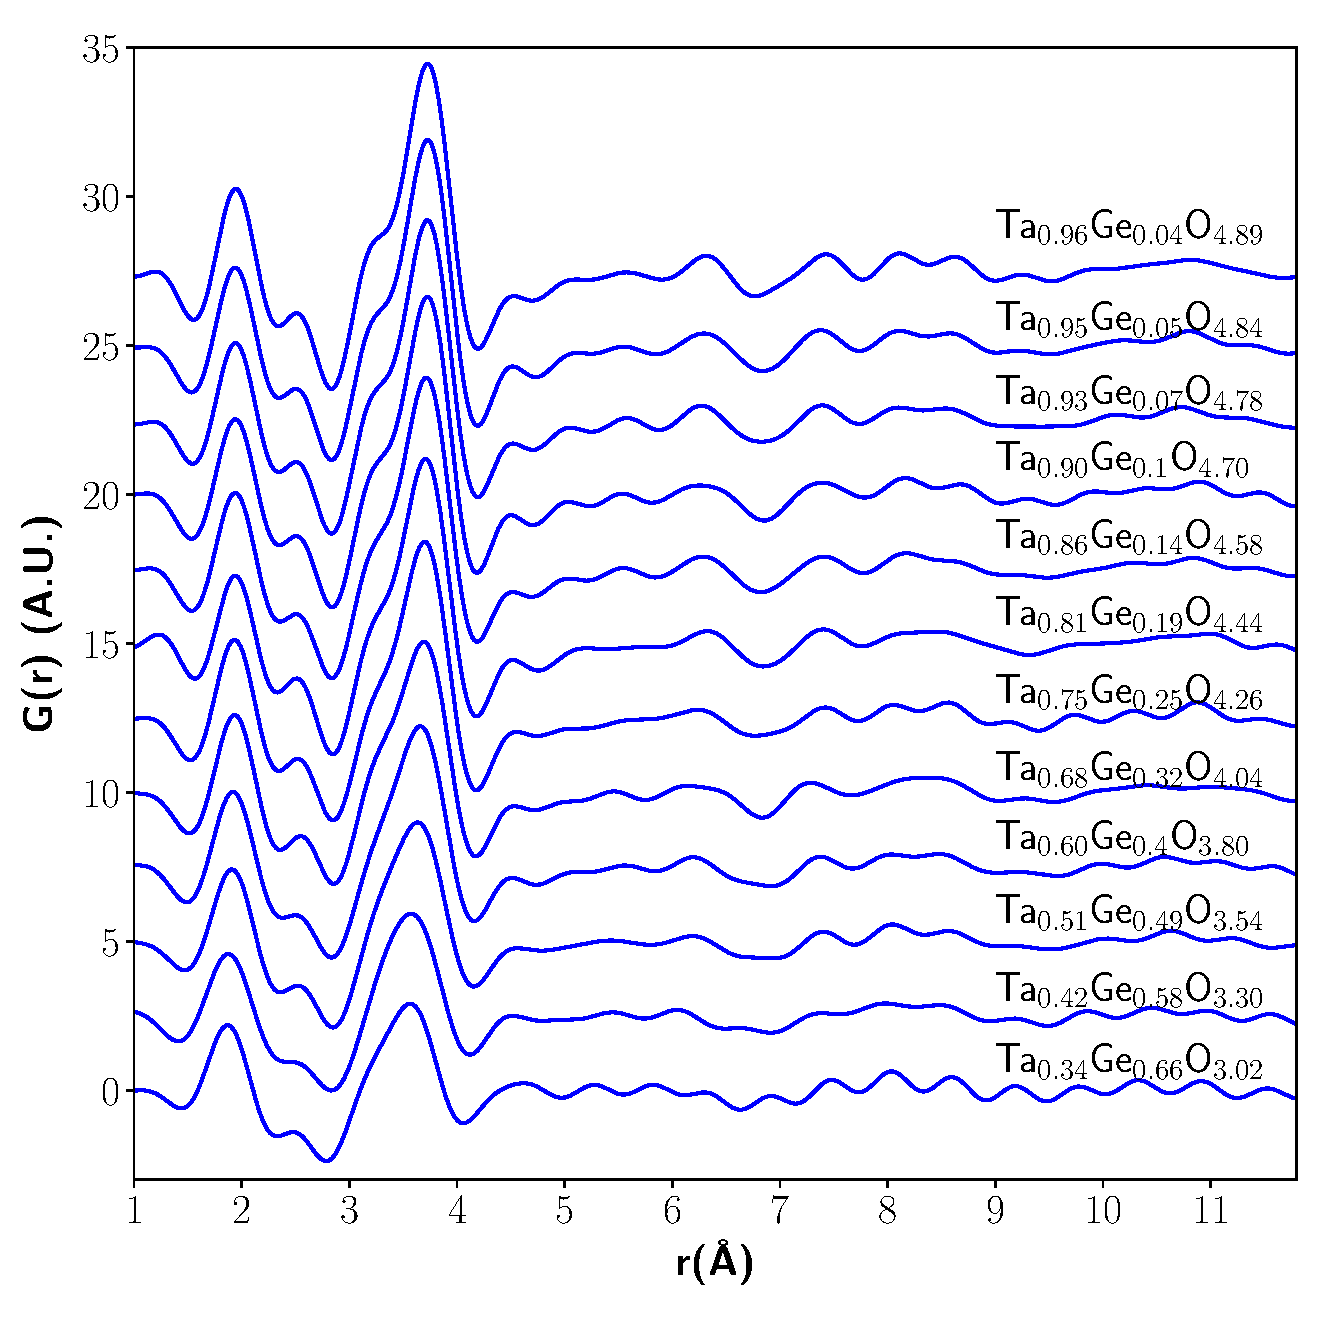
\includegraphics[width=0.4\textwidth]{waterfall.eps}}

\subfloat[]{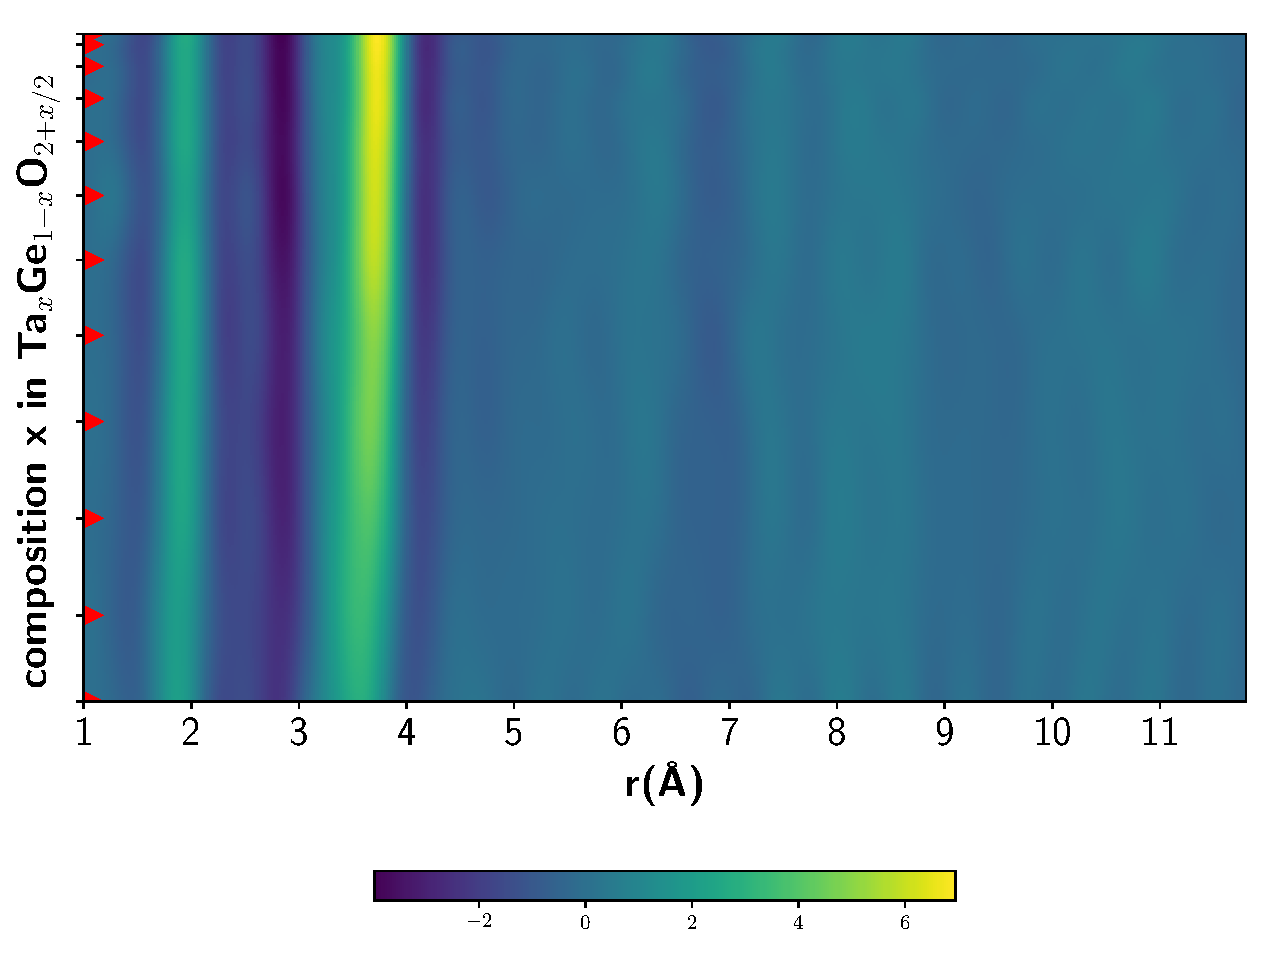
\includegraphics[width=0.9\linewidth]{contour.eps}}
\caption{(a) Waterfall plot of the PDFs generated using PDFgetX3 for Ta$_{x}$Ge$_{1-x}$O$_{2+x/2}$ compositions. The Ta cation composition $x$, increases from bottom to top. (b) A heatmap plot of the same set of PDFs as in (a). The color scale plot corresponds to the height of the PDF. Red arrows on the y-axis mark the specific compositions measured, while the compositions in-between are algorithmically interpolated.}
\label{fig:PDF}
\end{figure} 

\subsection{Uncovering structural trends of Ta$_{x}$Ge$_{1-x}$O$_{2+x/2}$ using EXAFS and PDF data}

\begin{figure*}[ht]
\centering
	\subfloat{\includegraphics[width=0.5\textwidth]{xas_mu.eps}}
	\hspace{-7ex}
	\subfloat{\includegraphics[width=0.5\textwidth]{exafs_chik.eps}}
	\hspace{-7ex}
	\subfloat{\includegraphics[width=0.5\textwidth]{exafs_chir.eps}}
	\caption{(a) The XAS absorption spectra of amorphous Ta$_{2}$O$_{5}$ and Ta$_{x}$Ge$_{1-x}$O$_{2+x/2}$ thin films. The spectra are vertically shifted for easier viewing. Film compositions are identical to those investigated in the PDF. The inset shows the variation of the unshifted L-III line with composition. (b) $\chi(k)$ and (c) $|\chi(R)|$ spectra as a function of composition. $|\chi(R)|$ is plotted without a phase shift. The top-most spectra for each figure corresponds to the spectra of pure Ta$_{2}$O$_{5}$.}
	\label{fig:xas}
\end{figure*}

XAS is a useful tool which probes the local structure and chemistry of materials and is particularly useful in investigating disordered systems. We take advantage of the chemical specificity of XAS to examine the Ta L-III edge to investigate the fine structure, or EXAFS centered around Ta atoms. The edge corresponds to dipole-allowed transitions 2p$_{3/2}\rightarrow$ 5d$_{5/2}$, 5d$_{3/2}$ (Figure \ref{fig:xas}a). There is no energy shift in the position of the white-line peak, which indicates that the formal valence of Ta is constant as Ge is incorporated into the amorphous structure. However, the height of the L-III edge decreases monotonically with Ge incorporation (Figure \ref{fig:xas}a inset). The height of the white-line peak directly correlates with d-orbital occupancy in 5d transition metals.\cite{Qi1987} Therefore, a decrease in the L-III edge peak suggests that Ge doping changes the d-band occupation of electrons i.e. Ta is being reduced. Reduction of the Ta atoms in the Ta$_{x}$Ge$_{1-x}$O$_{2+x/2}$ amorphous mixture is also reflected in X-ray photoelectron spectroscopy (XPS) spectra (not shown). Addition of GeO$_{2}$ causes the spin-orbit Ta $4f_{5/2}$ and Ta $4f_{7/2}$ doublet to shift to lower binding energies, a sign that is consistent with Ta becoming more metallic.

The behaviors of $k^{2}\chi(k)$ and its Fourier transform are plotted as a function of Ta cation composition in Figure \ref{fig:xas}. Here, $\chi(R)$ is not corrected for the photoelectron phase shift. The sample-to-sample variation of the $k^{2}\chi(k)$ spectra is difficult to interpret, so we limit ourselves to examining variations in the $\chi(R)$ spectra. We see that the position of the inner shell peak I is roughly independent of composition, whereas peak II changes in peak position and amplitude, though the exact behavior of the latter is hard to discern from the spectra alone. Other prominent features are the outer shell peaks III and IV, which show high variability in peak shape and position.  

We fit four experimental EXAFS spectra to amorphous structural models of similar compositions derived from \emph{ab-initio} genetic algorithms to gain a quantitative understanding of the EXAFS data. The resulting fit parameters are tabulated in Table \ref{table:exafs2} and the fitted EXAFS in $k$ and $R$-space are shown in Figure \ref{fig:exafs_fitted}. The combination of scattering paths yielding the lowest R-factor differ between each model, but generally consist of one or two inner-shell Ta-O single scattering paths, an outer shell Ta-Ta, or Ta-Ge single scattering path, and an outer shell Ta-O single scattering path. 

Our fits to pure Ta$_{2}$O$_{5}$ yield two Ta-O shells at 1.88 and 2.03 \AA \;(Table \ref{table:exafs2}), which shows the existence of two oxygen sites. These bond distances are close to our experimental results obtained from analysis of the PDF data (Figure \ref{fig:12f74}), although the PDF is only able to resolve a single Ta-O peak. By fixing the amplitude reduction factor to  $S_{o} = 1.0$, we estimated the coordination numbers in the EXAFS equation. We obtain $N = 2.92$ and $N = 1.20$ for the coordination numbers of the two Ta-O inner shells (Table \ref{table:exafs2}), hence the coordination number of the Ta-O inner shell is $N_{Ta-O} \sim 4$. This is lower than one might expect based on coordination numbers of crystalline Ta$_{2}$O$_{5}$, which is six or seven. \cite{Aleshina2002, Lee2013, Stephenson1971} However, the discrepancy is unsurprising if we consider the fact that the coordination number of metal-oxygen (M-O) complexes in amorphous melts and glasses can be significantly lower than in the corresponding crystalline phase, which holds true especially for cations with low fields and larger ionic radii i.e., poor network formers.\cite{Skinner2014} For comparison, we calculate the field strength of Ta-O and Ge-O as $F = Z_{M}/(r_{MO} - 1.24)^{2}$, where $Z_{M}$ is the formal charge of the cation, $r_{MO}$ is the M-O bond distance, and 1.24 is the ionic radius of Oxygen\cite{Shannon1969}. Using experimentally derived M-O bond distances we determine $F_{Ta_{2}O_{5}} = 10.5$ $e^{2}/\text{\AA}$ and $F_{GeO_{2}} = 16.7$ $e^{2}/\text{\AA}$. In contrast, $F_{SiO_{2}} = 26$ $e^{2}/\text{\AA}$.\cite{Skinner2014} Since Ta-O tends to be a poor network former, we expect the coordination numbers to be reduced and indeed our values are very much consistent with values from a recent EXAFS study by Bassiri et al.\cite{Bassiri2015} We also find the bond distances and coordination numbers for Ta-Ta and the outer shell Ta-O to be consistent with values obtained from the PDF and by Bassiri et al.\cite{Bassiri2015} 

%
%Note to me: I've gotten to here but need to think carefully about the rest of the paper. -Bruce, 3/25/2018
%

\begin{table}[ht]
\centering
\setlength{\tabcolsep}{5pt}
\begin{tabular}{llcccc}
\hline\hline
Model & Path & $R$(\AA) 
& $\Delta R$(\AA) & $N$ & $\sigma^{2}$ (\AA$^{2}$) \\
\hline
{} & Ta-O  			   	   & 1.88  & { }0.058 & 2.92 & 0.004 \\ 
Ta$_{2}$O$_{5}$	   & Ta-O  & 2.03  & { }0.047 & 1.20 & 0.004 \\ 
(Ta$_{16}$O$_{40}$)& Ta-Ta & 3.10  &   -0.001 & 1.05 & 0.005 \\
{} & Ta-O  			   	   & 3.53  &   -0.240 & 2.60 & 0.007 \\
{} & Ta-Ta 			   	   & 3.74  &   -0.001 & 0.21 & 0.005 \\
\hline
{}								   & Ta-O  & 1.91 &   -0.020 & 3.93 & 0.006 \\ 
Ta$_{0.93}$Ge$_{0.07}$O$_{\delta}$ & Ta-O  & 2.07 & { }0.067 & 0.80 & 0.006 \\
(Ta$_{15}$Ge$_{1}$O$_{40}$)		   & Ta-Ta & 3.10 &   -0.280 & 0.43 & 0.001 \\
{} 								   & Ta-O  & 3.52 &   -0.051 & 2.78 & 0.008 \\
\hline 
{}& Ta-O  									& 1.92 &   -0.051 & 4.13 & 0.006  \\ 
Ta$_{0.75}$Ge$_{0.25}$O$_{\delta}$	& Ta-O  & 2.11 & { }0.041 & 1.69 & 0.006  \\
(Ta$_{12}$Ge$_{4}$O$_{40}$) 		& Ta-Ta & 3.02 &   -0.257 & 6.17 & 0.011  \\
{}& Ta-Ge 									& 3.07 &   -0.084 & 12.7 & 0.020  \\
\hline 
{} & Ta-O   							 	& 1.93 & { }0.071 & 5.48 & 0.008 \\ 
Ta$_{0.51}$Ge$_{0.49}$O$_{\delta}$ & Ta-O   & 2.20 & { }0.093 & 1.79 & 0.008 \\
(Ta$_{8}$Ge$_{8}$O$_{40}$)		   & Ta-Ge  & 3.03 &   -0.008 & 7.99 & 0.018 \\
{} & Ta-Ta  							 	& 3.06 &   -0.060 & 14.2 & 0.023 \\
\hline 
\end{tabular}
\caption{EXAFS fit parameters for Ta$_{2}$O$_{5}$ and Ta$_{x}$Ge$_{1-x}$O$_{2+x/2}$ amorphous thin films on silicon nitride for four different compositions. Experimentally derived compositions are indicated without parenthesis, while the compositions of models derived from simulations are shown with parenthesis.}
\label{table:exafs2}
\end{table}

\begin{figure*}[t]
\centering
	\subfloat{\includegraphics[width=0.4\textwidth]{exafs_ta2o5.eps}}
	\hspace{-8ex}
	\subfloat{\includegraphics[width=0.4\textwidth]{exafs_ta15.eps}}
	\qquad
	\subfloat{\includegraphics[width=0.4\textwidth]{exafs_ta12.eps}}
	\hspace{-8ex}
	\subfloat{\includegraphics[width=0.4\textwidth]{exafs_ta8.eps}}
	\caption{Fitted EXAFS $\chi$(k) and $\chi$(R) spectra for (a) pure Ta$_{2}$O$_{5}$ (b) Ta$_{15}$Ge$_{1}$O$_{40}$ (c) Ta$_{12}$Ge$_{4}$O$_{40}$ and (d) Ta$_{8}$Ge$_{8}$O$_{40}$. The dashed lines are the best fit lines for each spectrum.}
	\label{fig:exafs_fitted}
\end{figure*}

The addition of GeO$_{2}$ into Ta$_{2}$O$_{5}$ result in conspicuous changes to pair bond distances. We present the inner shell Ta(Ge)-O bond distances based on our PDF data, $r_{Ta(Ge)-O}^{PDF}$, in Figure \ref{fig:exafs_all}a, while the Ta-O, Ta-Ta, and Ta-Ge inner shell bond distances obtained from our fits to the EXAFS spectra - $r_{Ta-O_{(I,II)}}^{EXAFS}$, $r_{Ta-Ta}^{EXAFS}$, $r_{Ta-Ge}^{EXAFS}$ - is shown in Figure \ref{fig:exafs_all}b. We note that $r_{Ta(Ge)-O}^{PDF}$ is assumed to be composed of overlapping inner shell Ta-O and Ge-O peaks, for which the contribution from the individual peaks depends on the composition. Comparing the PDF data in Figure \ref{fig:exafs_all}a to the EXAFS data in Figure \ref{fig:exafs_all}b, we notice that $r_{Ta-O_{(I,II)}}^{EXAFS}$ is actually increasing with the addition of GeO$_{2}$, where the increase is most prominent in the second inner shell Ta-O bond distance ($r_{Ta-O_{(II)}}^{EXAFS}$); the first inner shell Ta-O bond distance ($r_{Ta-O_{(I)}}^{EXAFS}$) shows a modest increase with decreasing $x$. For example, $r_{Ta-O_{(I)}}^{EXAFS}$ increases from 1.88 \AA\ to 1.91 \AA\ and $r_{Ta-O_{(II)}}^{EXAFS}$ increases from 2.03 \AA\ to 2.07 \AA\ when $x$ decreases from 1.0 to 0.93. However, the net effect of the change in $r_{Ta-O_{(I,II)}}^{EXAFS}$ results in a less drastic enhancement of $r_{Ta(Ge)-O}^{PDF}$ above linear interpolation of endmember values - at $x = 0.93$ $r_{Ta(Ge)-O}^{PDF}$ is 1.94 \AA. Assuming the contribution of the Ge-O PDF peak to $r_{Ta(Ge)-O}^{PDF}$ is negligible for Ta-rich compositions, the lack of a larger increase in $r_{Ta(Ge)-O}^{PDF}$ implies that the Ta-O structural unit experiences on average, only modest levels of distortions with low levels of GeO$_{2}$ doping.

\begin{figure*}[t]
\centering
	\subfloat{\includegraphics[width=0.4\textwidth]{ta-o.eps}}
	\hspace{-2ex}
	\subfloat{\includegraphics[width=0.4\textwidth]{ta-ta.eps}}
	\qquad
	\subfloat{\includegraphics[width=0.4\textwidth]{N.eps}}
	\hspace{-2ex}
	\subfloat{\includegraphics[width=0.4\textwidth]{oo_distance.eps}}
	\caption{
	(a) Composition dependence of Ta(Ge)-O bond distances determined from PDF data (first peaks in Figure \ref{fig:PDF}a). The solid line is an interpolation between values of endmembers.
	(b) Composition dependent bond distances determined from EXAFS data for Ta-O, Ta-Ta and Ta-Ge.
	(c) Composition dependent coordination numbers determined from EXAFS data for Ta-O, Ta-Ta and Ta-Ge.
	(d) Composition dependence of O-O bond distances determined from PDF data (second peaks in Figure \ref{fig:PDF}a). 
	}
	\label{fig:exafs_all}
\end{figure*}  

Further addition of GeO$_{2}$ in Ta$_{2}$O$_{5}$ results in decrease of $r_{Ta(Ge)-O}^{PDF}$ even as $r_{Ta-O_{(I,II)}}^{EXAFS}$ continues to increase. We presume that the decrease in $r_{Ta(Ge)-O}^{PDF}$ with decreasing $x$ is the result of increasing contributions from the Ge-O peak to $r_{Ta(Ge)-O}^{PDF}$, though without explicit knowledge of the Ge-O bond distance ($r_{Ge-O}$) it is difficult to reach a definitive conclusion. $r_{Ta-Ta}^{EXAFS}$ and $r_{Ta-Ge}^{EXAFS}$ in contrast do not experience substantial changes with change in x (Figure \ref{fig:exafs_all}b). The Ta-Ta pair bond distance experiences a slight contraction with decreasing $x$, though the sparseness of the data makes it difficult to infer a trend.

GeO$_{2}$ substitution also elicits a dramatic change in the coordination environment around Ta (Figure \ref{fig:exafs_all}c). Interestingly, as more GeO$_{2}$ is substituted we see an increase in the Ta-O coordination number. Ge occupation of Ta$_{2}$O$_{5}$ interstitial sites may lead to increased network connectivity and in turn, increase Ta-O coordination. The most dramatic coordination shift however, occurs for the metal-metal (M-M) pairs, namely Ta-Ta and Ta-Ge. We observe a large coordination increase in the Ta-Ta coordination ($N_{Ta-Ta}$) from $x = 0.93$ to $x = 0.75$, where $N_{Ta-Ta}$ jumps from 0.43 to 6.17. The EXAFS fit at $x = 0.75$ also includes a Ta-Ge shell with a large coordination number of $N_{Ta-Ge} = 12.7$. When the composition of Ta and Ge cations are roughly equal, the short-range order starts to resemble that of low temperature Ta$_{2}$O$_{5}$ (L-Ta$_{2}$O$_{5}$). This is evidenced by the coordination number of the Ta-O inner shells ($N_{Ta-O_{(I, II)}}$), where $N_{Ta-O_{(I)}} = 5.48$ and $N_{Ta-O_{(II)}} = 1.79$ (collectively $N_{Ta-O} \sim 7$ for the inner shell). Moreover, the M-M pair coordination numbers experiences an inversion, where $N_{Ta\_Ta}$ becomes large than $N_{Ta\_Ge}$. This suggests that there may be some segregation occurring at the atomic level.  

We can use our findings from this study to elucidate trends from previous studies on amorphous Ta$_{x}$Ge$_{1-x}$O$_{2+x/2}$ thin films.\cite{Naoi2018jap} Specifically, we wish to address the 1) large decrease in density away from linear interpolation of endmembers in the 0.6 $<$ $x$ $<$ 0.9 Ta cation range and 2) the dielectric enhancement observed in the 0.75 $<$ $x$ $<$ 0.95. 

First, we attribute the reduction of density in the specified range to increases in bond distances. Bond distances relate inversely with density: an increase in bond distances will typically result in decreased density. 
Our data is consistent with this expectation: the enhancement of $r_{Ta(Ge)-O}^{PDF}$ above linear interpolation should result in a proportional decrease in density for a given $x$. Also note the overall increase in $r_{O-O}$ with decreasing $x$. This suggests a distortion in the M-O-M structural unit, which may further contribute to local bond distance expansion.

Second, we suggest that changes in the local coordination environment around Ta brought about by substitution of GeO$_{2}$ play a role in dielectric enhancement. Prominent features supporting this claim are the sizable shifts in Ta-Ge and Ta-Ta coordination (Figure \ref{fig:exafs_all}c), accompanied by changes in O-O pair bond distances (Figure \ref{fig:exafs_all}d). Though the data for Ta-Ge coordination is sparse, the jump in Ta-Ge coordination - from $N_{Ta\_Ge} = 7.99$ at $x = 0.5$ to $N_{Ta\_Ge} = 12.7$ for $x = 0.75$ - clearly coincides with the transition from the unenhanced to enhanced region, where the transition roughly occurs around $x \sim 0.7$.\cite{Naoi2018jap} The corresponding drop in $N_{Ta\_Ta}$ from $x = 0.5$ to $x = 0.75$ is likely due to reorganization of the local environment such that there is a high Ge occupancy around Ta instead of Ta. We suspect that the reorganization continues to occur in the enhanced region ($x = 0.75$ and $x = 0.93$), which is partially indicated by the further drop of $N_{Ta\_Ta}$. The O-O bond distances obtained from PDF data provides some evidence of reorganization between $x = 0.75$ and $x = 0.93$ where coordination data from EXAFS is lacking. We observe a significant increase in $r_{O-O}$ from roughly $x = 0.75$ to $x = 0.85$, with a peak at roughly $x \sim 0.85$; further increase in $x$ above $x = 0.85$ result in the decrease of the O-O bond distance (Figure \ref{fig:exafs_all}d). We surmise that local atomic reorganization occurring between 0.5 $<$ $x$ $<$ 0.93 creates local deviations in stoichiometry (for instance Ge interstitials), enhancing low-frequency polarizabilities and in turn enhance the dielectric constants. Nonetheless, a careful probe of the local environment around Ge, whether it be through EXAFS, PDF, or some other technique, along with measurements of the IR spectra in the enhanced region should yield a more comprehensive picture of the relationship between the low-frequency phonons modes and the local atomic structure. 

\section{Conclusion}
We have investigated the local structure of amorphous Ta$_{2}$O$_{5}$ and Ta$_{x}$Ge$_{1-x}$O$_{2+x/2}$ thin films using PDF, EXAFS, and MD. The films were sputtered on silicon nitride films to facilitate the background subtraction process, yielding data of very high quality. Reliable distribution functions for both Ta$_{2}$O$_{5}$ and Ta$_{x}$Ge$_{1-x}$O$_{2+x/2}$ could be inferred from the diffraction patterns. The results of PDF analysis were combined with EXAFS to interpret the local structure evolution of Ta$_{x}$Ge$_{1-x}$O$_{2+x/2}$ with changes in composition. The coordination numbers and bond distances of amorphous Ta$_{2}$O$_{5}$ are consistent with values reported in previous studies, while addition of GeO$_{2}$ in Ta$_{2}$O$_{5}$ clearly resulted in substantial alterations to the local environment of pure Ta$_{2}$O$_{5}$. We deduce that bond distance enhancement is directly responsible for suppressions of density observed previously. Finally, we explain the previously observed enhancement in the dielectric constant as a direct consequence of changes in local coordination, which we presume enhances the low-frequency vibrational modes. Direct measurement of these low-frequency modes is needed to confirm our hypothesis.

\begin{acknowledgments}
%updated 3/25/2018; RBvD
This work was supported by the U.S. Department of Energy under Grant No. DE-FG02-06ER06-15. This work was performed in part at the Cornell NanoScale Facility, a member of the National Nanotechnology Infrastructure Network, which is supported by the National Science Foundation under Grant No. Grant ECS-15420819. This work is based upon research conducted at the Cornell High Energy Synchrotron Source (CHESS) which is supported by the National Science Foundation and the National Institutes of Health/National Institute of General Medical Sciences under NSF award DMR-1332208. This work made use of the Cornell Center for Materials Research Shared Facilities which are supported through the NSF MRSEC program (DMR-1719875).
\end{acknowledgments}

% REFERENCES
\bibliography{library}

\end{document}
% ***** End ******